The forward kinematics of the manipulator are described by the equations below, where the reference coordinate frames are given by \emph{Figure \ref{fig:coords}}.
\begin{figure}[htp]
  \centering
  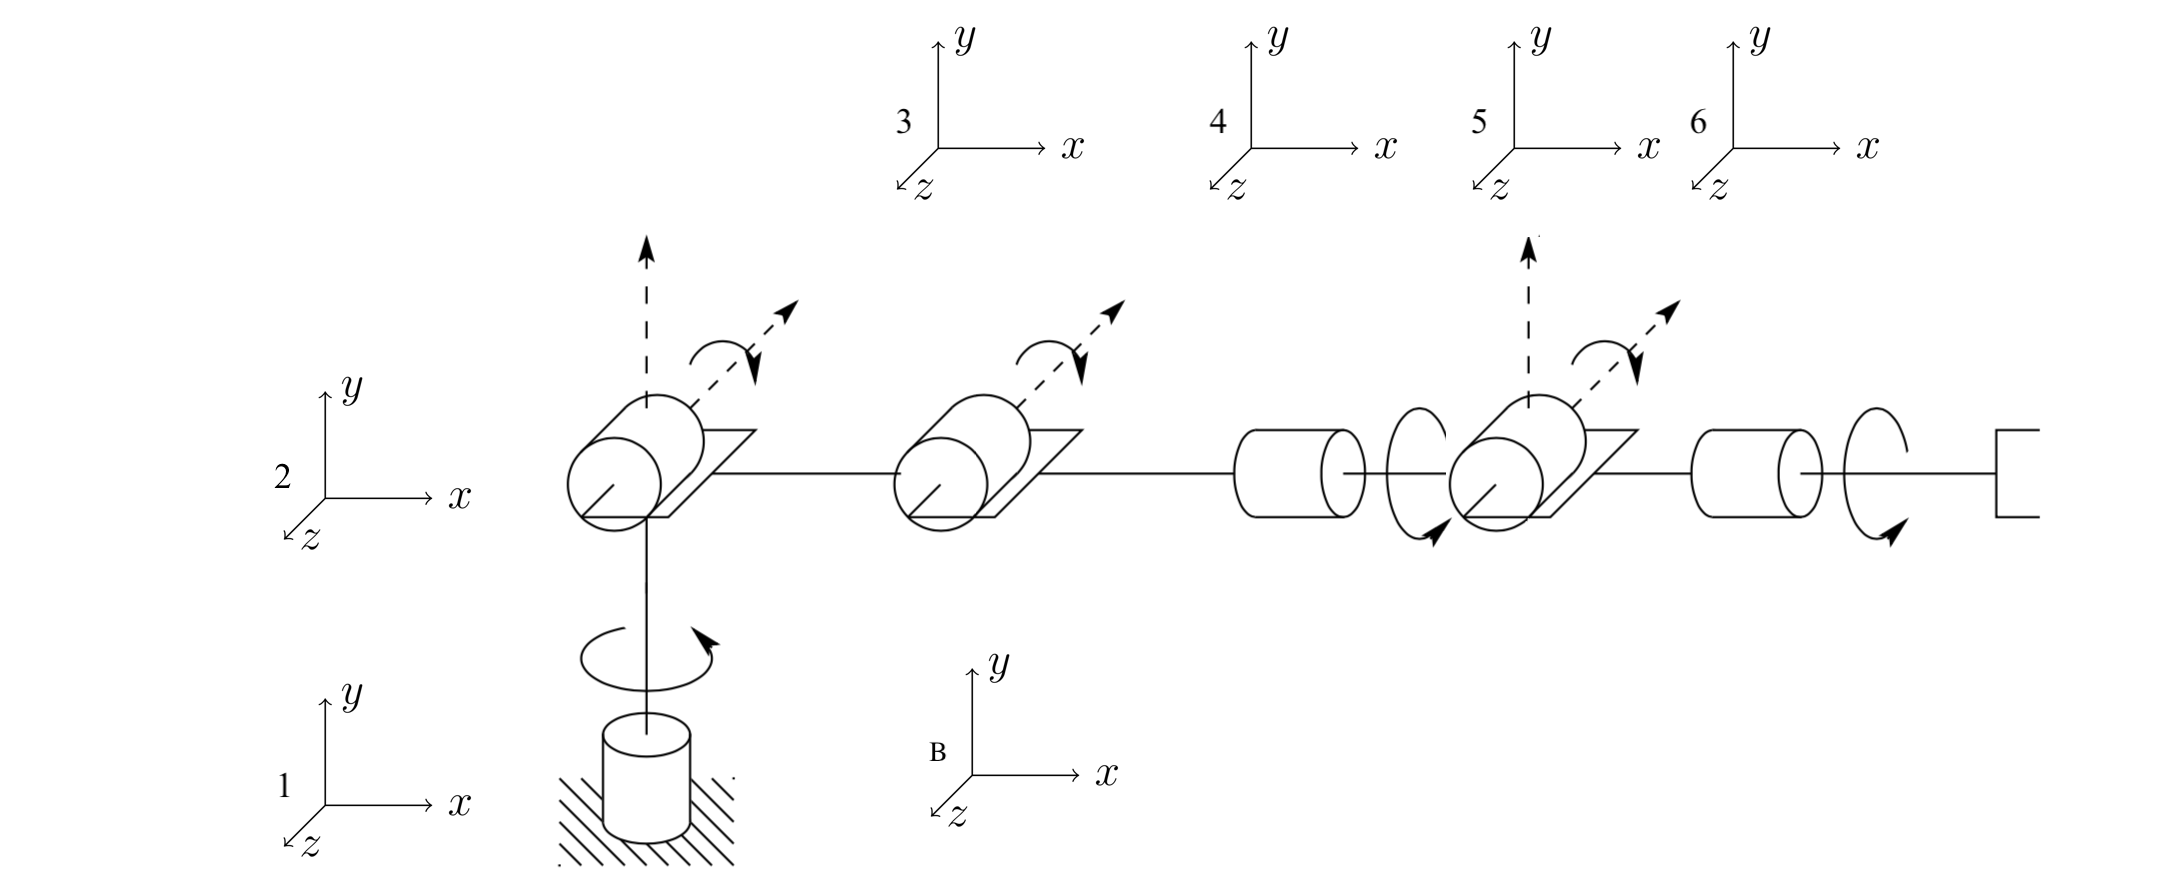
\includegraphics[width=.9\textwidth]{zero2}
  \caption{Coordinate Systems}
  \label{fig:coords}
\end{figure}

Given the lengths of each of the manipulator links,
\[
\begin{aligned}
  ^I_Br_1 = \begin{bmatrix} 0\\0\\ \ell_b\end{bmatrix} & \quad
  ^1_1r_2 = \begin{bmatrix} 0\\0\\ \ell_1\end{bmatrix} & \quad
  ^2_2r_3 = \begin{bmatrix} 0\\\ell_2\\ 0\end{bmatrix} & \quad
  ^3_3r_4 = \begin{bmatrix} 0\\\ell_3\\ 0\end{bmatrix} & \quad
  ^4_4r_5 = \begin{bmatrix} 0\\\ell_4\\ 0\end{bmatrix} & \quad
  ^5_5r_6 = \begin{bmatrix} 0\\\ell_5\\ 0\end{bmatrix} & \quad
\end{aligned}
\]
The position of each link relative to the inertial frame is given as:
\[
\begin{aligned}
^I_Br_1 &= {}_Br_1 &\quad
^I_Br_2 &= r_1 + {}^IT_1 {}^1_1r_2 &\quad
^I_Br_3 &= r_2 + {}^IT_2 {}^2_2r_3 \\
^I_Br_4 &= r_3 + {}^IT_3 {}^3_3r_4 &\quad
^I_Br_5 &= r_4 + {}^IT_4 {}^4_4r_5 &\quad
^I_Br_6 &= r_5 + {}^IT_5 {}^5_5r_6
\end{aligned}
\]

\[
\begin{aligned}
  ^I_Br_1 =&
  \begin{bmatrix}
    0\\ 0\\ \ell_b
  \end{bmatrix} & \quad
  ^I_Br_2 =
  \begin{bmatrix}
    0\\ 0\\ \ell_b + \ell_1
  \end{bmatrix} & \quad
  ^I_Br_3 =
  \begin{bmatrix}
    -\ell_2c_{\theta_2}s_{\theta_1}\\
    \ell_2c_{\theta_{12}}\\
    \ell_b+\ell_1+\ell_2s_{\theta_2}
  \end{bmatrix} & \quad
  ^I_Br_4 =
  \begin{bmatrix}
    -s_{\theta_1}(\ell_3c_{\theta_{23}} + \ell_2c_{\theta_2}) \\
    c_{\theta_1}(\ell_3c_{\theta_{23}} + \ell_2c_{\theta_2}) \\
    \ell_1 + \ell_b + \ell_3s_{\theta_{23}} + \ell_2s_{\theta_2}
  \end{bmatrix} \\
\end{aligned}
  \]
  \[
  ^I_Br_5 =
  \begin{bmatrix}
    -s_{\theta_1}(\ell_3c_{\theta_{23}} + \ell_4c_{\theta_{23}} + \ell_2c_{\theta_2}) \\
    c_{\theta_1}(\ell_3c_{\theta_{23}} + \ell_4c_{\theta_{23}} + \ell_2c_{\theta_2}) \\
    \ell_1 + \ell_b + \ell_3s_{\theta_{23}} + \ell_4s_{\theta_{23}} + \ell_2s_{\theta_2}
  \end{bmatrix}
  \]
  \[
  ^I_Br_6 =
  \begin{bmatrix}
  \begin{aligned}
      &\ell_5c_{\theta_1}s_{\theta_4}s_{\theta_5} - \ell_4c_{\theta_{23}}s_{\theta_1} - \ell_2c_{\theta_2}s_{\theta_1} - \ell_5c_{\theta_{23}}c_{\theta_5}s_{\theta_1} - \ell_3c_{\theta_{23}}s_{\theta_1} \\
      &\qquad\qquad+ \ell_5c_{\theta_2}c_{\theta_4}s_{\theta_1}s_{\theta_3}s_{\theta_5} + \ell_5c_{\theta_3}c_{\theta_4}s_{\theta_1}s_{\theta_2}s_{\theta_5} \\
      &\ell_5(s_{\theta_5}(s_{\theta_1}s_{\theta_4} - c_{\theta_4}(c_{\theta_1}c_{\theta_2}s_{\theta_3} + c_{\theta_1}c_{\theta_3}s_{\theta_2})) - c_{\theta_5}(c_{\theta_1}s_{\theta_2}s_{\theta_3} - c_{\theta_1}c_{\theta_2}c_{\theta_3})) \\
      &\qquad\qquad -\ell_3(c_{\theta_1}s_{\theta_2}s_{\theta_3} - c_{\theta_1}c_{\theta_2}c_{\theta_3}) -\ell_4(c_{\theta_1}s_{\theta_2}s_{\theta_3} - c_{\theta_1}c_{\theta_2}c_{\theta_3}) + \ell_2c_{\theta_1}c_{\theta_2} \\
      &\ell_1 + \ell_b + \ell_3s_{\theta_{23}} + \ell_4s_{\theta_{23}} + \ell_2s_{\theta_2} + \dfrac{\ell_5c_{\theta_{23}}s_{\theta_{45}}}{2} + \ell_5s_{\theta_{23}}c_{\theta_5} - \dfrac{\ell_5s_{\theta_4 - \theta_5}c_{\theta_{23}}}{2}
    \end{aligned}
  \end{bmatrix}
\]
\newpage
Given the direction cosine matrices,

\[
rotx(\theta) = \begin{bmatrix}
 1 & 0 & 0\\
 0 & \cos(\theta) & -\sin(\theta) \\
 0 & \sin(\theta) & \cos(\theta)
\end{bmatrix}~,\quad
roty(\theta) = \begin{bmatrix}
 1 & 0 & 0\\
 0 & \cos(\theta) & -\sin(\theta) \\
 0 & \sin(\theta) & \cos(\theta)
\end{bmatrix}
\]
\[
rotz(\theta) = \begin{bmatrix}
 \cos(\theta) & 0 & \sin(\theta)\\
  0 & 1 & 0 \\
 -\sin(\theta) & \cos(\theta) & 0
\end{bmatrix}
\]
The orientation of each link with respect to the inertial frame is given as:
\[
\begin{aligned}
^IT_1 &= rotz(\theta_1) \\
^IT_2 &= rotz(\theta_1)~rotx(\theta_2)\\
^IT_3 &= rotz(\theta_1)~rotx(\theta_2)~rotx(\theta_3)\\
^IT_4 &= rotz(\theta_1)~rotx(\theta_2)~rotx(\theta_3)~roty(\theta_4)\\
^IT_5 &= rotz(\theta_1)~rotx(\theta_2)~rotx(\theta_3)~roty(\theta_4)~rotx(\theta_5)\\
^IT_6 &= rotz(\theta_1)~rotx(\theta_2)~rotx(\theta_3)~roty(\theta_4)~rotx(\theta_5)~roty(\theta_6)\\
\end{aligned}
\]
\[
\begin{aligned}
  ^IT_1 =
  \begin{bmatrix}
    c_{\theta_1}& -s_{\theta_1}& 0\\
    s_{\theta_1}&  c_{\theta_1}& 0\\
    0&            0& 1\\
  \end{bmatrix} & \quad
  ^IT_2 =
  \begin{bmatrix}
    c_{\theta_1}& -c_{\theta_2}s_{\theta_1}&  s_{\theta_1}s_{\theta_2}\\
    s_{\theta_1}&  c_{\theta_1}c_{\theta_2}& -c_{\theta_1}s_{\theta_2}\\
    0&              s_{\theta_2}&              c_{\theta_2}\\
  \end{bmatrix} & \quad
  ^IT_3 =
  \begin{bmatrix}
    c_{\theta_1}& -c_{\theta_{23}}s_{\theta_1}&  s_{\theta_{23}}s_{\theta_1}\\
    s_{\theta_1}&  c_{\theta_{23}}c_{\theta_1}& -s_{\theta_{23}}c_{\theta_1}\\
    0&              s_{\theta_{23}}&              c_{\theta_{23}}\\
  \end{bmatrix}
\end{aligned}
\]
\[
^IT_4 =
\begin{bmatrix}
c_{\theta_1}c_{\theta_4} - s_{\theta_{23}}s_{\theta_1}s_{\theta_4}& -c_{\theta_{23}}s_{\theta_1}& c_{\theta_1}s_{\theta_4} + s_{\theta_{23}}c_{\theta_4}s_{\theta_1}\\
c_{\theta_4}s_{\theta_1} + s_{\theta_{23}}c_{\theta_1}s_{\theta_4}&  c_{\theta_{23}}c_{\theta_1}& s_{\theta_1}s_{\theta_4} - s_{\theta_{23}}c_{\theta_1}c_{\theta_4}\\
-c_{\theta_{23}}s_{\theta_4}&              s_{\theta_{23}}&                                       c_{\theta_{23}}c_{\theta_4}\\
\end{bmatrix}
\]
\[
^IT_5 =
\begin{bmatrix}
c_{\theta_1}c_{\theta_4} - s_{\theta_{23}}s_{\theta_1}s_{\theta_4}& s_{\theta_5}(c_{\theta_1}s_{\theta_4} + s_{\theta_{23}}c_{\theta_4}s_{\theta_1}) - c_{\theta_{23}}c_{\theta_5}s_{\theta_1}& c_{\theta_5}(c_{\theta_1}s_{\theta_4} +
 s_{\theta_{23}}c_{\theta_4}s_{\theta_1}) + c_{\theta_{23}}s_{\theta_1}s_{\theta_5}\\
c_{\theta_4}s_{\theta_1} + s_{\theta_{23}}c_{\theta_1}s_{\theta_4}& s_{\theta_5}(s_{\theta_1}s_{\theta_4} - s_{\theta_{23}}c_{\theta_1}c_{\theta_4}) + c_{\theta_{23}}c_{\theta_1}c_{\theta_5}& c_{\theta_5}(s_{\theta_1}s_{\theta_4} - s_{\theta_{23}}c_{\theta_1}c_{\theta_4}) - c_{\theta_{23}}c_{\theta_1}s_{\theta_5}\\
-c_{\theta_{23}}s_{\theta_4}&                                                     s_{\theta_{23}}c_{\theta_5} + c_{\theta_{23}}c_{\theta_4}s_{\theta_5}&                                                     c_{\theta_{23}}c_{\theta_4}c_{\theta_5} - s_{\theta_{23}}s_{\theta_5}\\
\end{bmatrix}
\]
\[
^IT_6 =
\begin{bmatrix}
  ^IT_{6(1,1)} & ^IT_{6(1,2)} & ^IT_{6(1,3)}\\
  ^IT_{6(2,1)} & ^IT_{6(2,2)} & ^IT_{6(2,3)}\\
  ^IT_{6(3,1)} & ^IT_{6(3,2)} & ^IT_{6(3,3)}\\
\end{bmatrix}
\]
\[
\begin{aligned}
^IT_{6(1,1)} &=
c_{\theta_6}(c_{\theta_1}c_{\theta_4} - s_{\theta_{23}}s_{\theta_1}s_{\theta_4}) - s_{\theta_6}(c_{\theta_5}(c_{\theta_1}s_{\theta_4} + s_{\theta_{23}}c_{\theta_4}s_{\theta_1}) + c_{\theta_{23}}s_{\theta_1}s_{\theta_5})\\
^IT_{6(1,2)} &=
s_{\theta_5}(c_{\theta_1}s_{\theta_4} + s_{\theta_{23}}c_{\theta_4}s_{\theta_1}) - c_{\theta_{23}}c_{\theta_5}s_{\theta_1}\\
^IT_{6(1,3)} &=
c_{\theta_6}(c_{\theta_5}(c_{\theta_1}s_{\theta_4} + s_{\theta_{23}}c_{\theta_4}s_{\theta_1}) + c_{\theta_{23}}s_{\theta_1}s_{\theta_5}) + s_{\theta_6}(c_{\theta_1}c_{\theta_4} - s_{\theta_{23}}s_{\theta_1}s_{\theta_4})\\
^IT_{6(2,1)} &=
c_{\theta_6}(c_{\theta_4}s_{\theta_1} + s_{\theta_{23}}c_{\theta_1}s_{\theta_4}) - s_{\theta_6}(c_{\theta_5}(s_{\theta_1}s_{\theta_4} - s_{\theta_{23}}c_{\theta_1}c_{\theta_4}) - c_{\theta_{23}}c_{\theta_1}s_{\theta_5})\\
^IT_{6(2,2)} &=
s_{\theta_5}(s_{\theta_1}s_{\theta_4} - s_{\theta_{23}}c_{\theta_1}c_{\theta_4}) + c_{\theta_{23}}c_{\theta_1}c_{\theta_5}\\
^IT_{6(2,3)} &=
s_{\theta_6}(c_{\theta_4}s_{\theta_1} + s_{\theta_{23}}c_{\theta_1}s_{\theta_4}) + c_{\theta_6}(c_{\theta_5}(s_{\theta_1}s_{\theta_4} - s_{\theta_{23}}c_{\theta_1}c_{\theta_4}) - c_{\theta_{23}}c_{\theta_1}s_{\theta_5})\\
^IT_{6(3,1)} &=
s_{\theta_6}(s_{\theta_{23}}s_{\theta_5} - c_{\theta_{23}}c_{\theta_4}c_{\theta_5}) - c_{\theta_{23}}c_{\theta_6}s_{\theta_4}\\
^IT_{6(3,2)} &=
s_{\theta_{23}}c_{\theta_5} + c_{\theta_{23}}c_{\theta_4}s_{\theta_5}\\
^IT_{6(3,3)} &=
c_{\theta_6}(s_{\theta_{23}}s_{\theta_5} - c_{\theta_{23}}c_{\theta_4}c_{\theta_5}) - c_{\theta_{23}}s_{\theta_4}s_{\theta_6}
\end{aligned}
\]
